%! Author = mariuszindel
%! Date = 25.01.21

\section{Wahrscheinlichkeit}



\subsection{Wahrscheinlichkeitsrechnung}

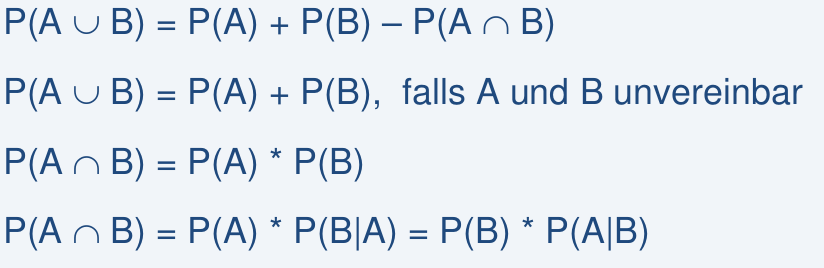
\includegraphics[width=\linewidth]{graphic/extern-reto/Wahrscheinlichkeit.png}

\subsubsection{Laplace}
\colorbox{lightlightgrey}{$P(A)=\frac{\text { Anzahl der guenstigen Ergebnisse } A}{\text { Anzahl aller Ergebnisse } \Omega}=\frac{|A|}{|\Omega|}=\frac{|A|}{n}$}

\subsubsection{Lotto}
\colorbox{lightlightgrey}{$\frac{\binom{Gezogene}{Treffer} * \binom{Nicht-Gezogene}{Falsche}}{Anzahl aller Ergebnisse}$}\\


\subsection{Kombinatorik}

\subsubsection{Geordnete Proben}
Die Anzahl der  k-Tupel aus einer n-Menge \textcolor{subsectioncolor}{mit Wiederholung} ist: \colorbox{lightlightgrey}{$n^k$}\\
Die Anzahl der  k-Tupel aus einer n-Menge \textcolor{subsectioncolor}{ohne Wiederholung} ist:\\
\colorbox{lightlightgrey}{$Anzahl =\frac{n !}{(n-k) !}$}\\
\textit{Beispiel:}\\
\textit{Beim Pferde-Toto “3 aus 18” muss man von 18 Pferden 3 gemäß der Reihenfolge ihres Zieleinlaufs tippen.}\\
$\rightarrow 18 \times 17 \times 16 = 4896$


\subsubsection{Geordnete Proben}
Die Anzahl der  k-elementigen Teilmengen aus einer n-elementigen Menge ist:\\
\colorbox{lightlightgrey}{$\left(\begin{array}{c}n \\ k\end{array}\right)=\frac{n !}{k !(n-k) !}$}

\textit{Beispiel:}\\
\textit{Eine Schulklasse mit 25 Schülern möchte ein Schachturnier austragen, bei dem jeder Schüler einmal gegen jeden anderen Schüler spielt. Wie viele Spiele werden ausgetragen?}\\
$\rightarrow \left(\begin{array}{c}25 \\ 2\end{array}\right)=\frac{25 \cdot 24}{2 !}=300$

\subsection{Bitfehler}
\colorbox{lightlightgrey}{$P(Fehlerhaft) = 1 - P(0 Fehler)$}\\
\colorbox{lightlightgrey}{$= 1 - $P(BitFehler)$^{Datenblock}$}



\subsection{Binominalverteilung}
Wie gross ist die Wahrscheinlichkeit, dass:
\begin{itemize}
    \item genau 3
    \item weniger als 3
\end{itemize}
\colorbox{lightlightgrey}{$P(X = k) = \binom{n}{k} p^k(1 - p)^{n-k}$}\\
Wenn z.B. $\le$ 3 gesucht ist, muss für (k = 0) + (k = 1) + (k = 2) + (k = 3) gerechnet werden.

\vfill
$$
\columnbreak